%!TEX root = ../thesis.tex
%*******************************************************************************
%****************************** Sixth Chapter **********************************
%*******************************************************************************
\chapter{Implementation}

\graphicspath{{Chapter6/Figs/Raster/}{Chapter6/Figs/}}

\section{Development Environment and Tools}

Specific systems and tools were used to build the demonstrator network and client applications. 
These choices and their explanations are detailed below, which could also be helpful in making this project reproducible.

\underline{Operating System}: Ubuntu

\underline{Version Control}: A version control system or software keeps track of source code modifications, 
so that developers can compare earlier versions of the code, revert changes, and 
minimise disruptions of mistakes \citep{atlassian2018vcs}. It is essential to medium to large scaled projects.

All work done at the implementation stage was tracked with the version control system Git. 
Git is a distributed version control system, where repositories can be backed up to a remote server, 
such as on the cloud. This is done with GitHub, a git-based version control, code hosting and 
project management service that offers free private repositories to verified students \citep{github2018education}.

\underline{Code Editor}: The Hyperledger Composer framework does not require a dedicated integrated 
development environment and recommends using a text editor. Visual Studio Code, an open source text editor developed 
by Microsoft was chosen as it has a dedicated syntax checking and beautifying official plugin for Hyperledger Composer.

\begin{figure}[!hb] 
    \centering    
    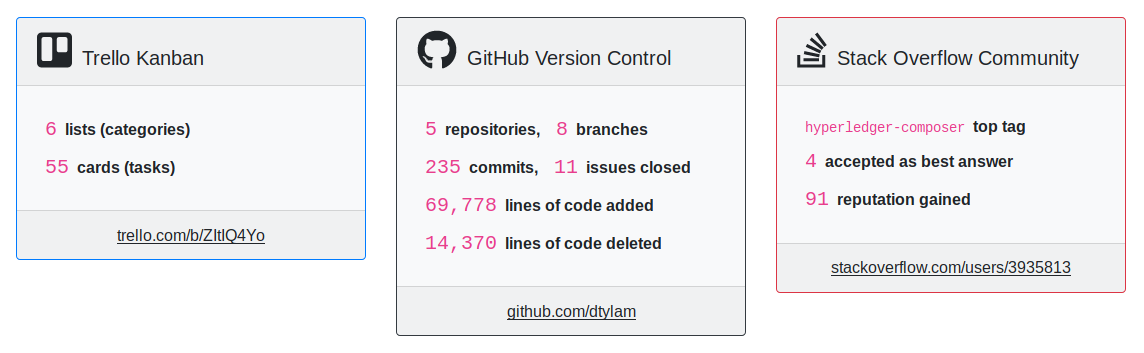
\includegraphics[width=1.0\textwidth]{platforms_stats}
    \caption[Project Management Statistics]
        {Statistics from Trello, GitHub and Stack Overflow collected over the duration of this project} 
    \label{fig:platforms_stats}
\end{figure}

\section{Architecture and Tech Stack}

\begin{figure}[!ht] 
    \centering    
    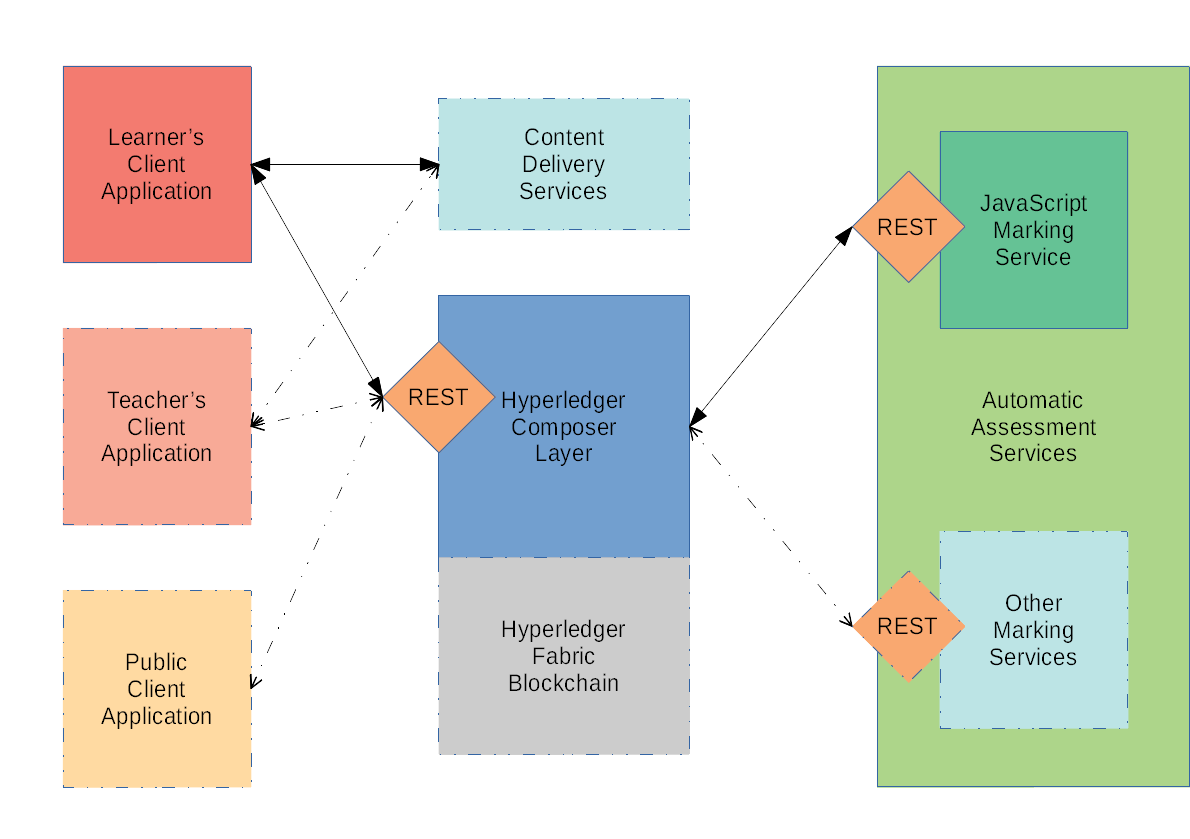
\includegraphics[width=1.0\textwidth]{architecture}
    \caption[Component architecture overview for the demonstrator system built]
        {Component architecture overview for the demonstrator system built}
    \label{fig:architecture}
\end{figure} 

\begin{figure}[!ht] 
    \centering    
    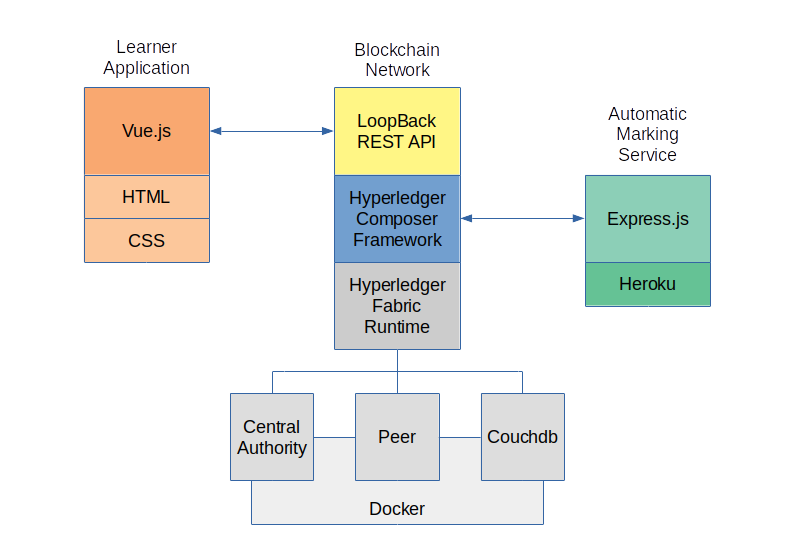
\includegraphics[width=0.9\textwidth]{techstack}
    \caption[Technology Stack overview for the demonstrator system built]
        {Technology Stack overview for the demonstrator system built}
    \label{fig:techstack}
\end{figure} 

\section{Docker and the Command Line Interface}

\section{Application Program Interface}

\section{Learner Client Application}

\section{Teacher Client Application}

